\documentclass[a4paper,12pt]{book} 
\usepackage{graphicx}
\usepackage{hyperref}
\usepackage{graphicx}
\graphicspath{{./Images/}}
\hypersetup{
	colorlinks=true,
	linkcolor=blue,
	filecolor=magenta,      
	urlcolor=cyan,
}




\begin{document} 
	
\title{Requirement Analysis and Specification Document RASD}
\author{KONG XIANGYI\and ZHANG YUEDONG}
\date{\today}


\frontmatter
\maketitle


\tableofcontents

\mainmatter

\chapter{Introduction} \label{C1:Introduction}

\section{Purpose}
This document is Requirement Analysis and Specification Document(RASD). The main purpose of this document is the following points
\begin{itemize}
	\item Communicates an understanding of the requirements to the audience and explains both the application domain and the system to be developed.
	\item Contractual: Make this project formal and written so that it has legal effect.
	\item As the baseline for project planning and estimation. i.e. size, cost, schedule. 
	\item As the baseline for software evaluation
		\subitem It can support system testing, verification and validation activities
		\subitem It should contain enough information to verify whether the delivered system meets requirements
	\item As the baseline for change control, such as requirements change, software evolves.
\end{itemize}
And this RASD has the following intended audiences
\begin{itemize}
	\item Costumers \& Users : Some user may interest in validating system goals and high-level description of functionalities.
	\item Systems and Requirements Analysts: The RASD may help them to write various specifications of other systems that inter-relate.
	\item Developers, Programmers: The RASD may help the to implement the requirements
	\item Testers: The RASD may help the to determine that the requirements have been met
	\item Project Managers: The RASD may help them to measure and control the analysis and development processes
\end{itemize}

\section{Scope}
\subsection{Description of the given problem}

At the end of 2019, a global epidemic broke out and swept almost all countries in the world in just a few months. Starting in 2020, people's life rhythm has been completely disrupted by this epidemic, a lot of cities are blocked, people are allowed to exit their homes only for essential needs, everyone had to wear masks and respect the social-distancing at least 1.5 m. In the public area, the human community has to take measures to avoid the crazy spread of the virus. Restaurants began to use dividers to separate the table, supermarkets and museums began to restrict flow of people, the school also adopted into two classes mode: online and onsite.

In this situation, a new problem arises, how to delay the spread of the virus through technical means? 

Since grocery shopping is the most needed activity under the lock-down, so let’s narrow the problem to grocery shopping.

In the supermarket, In order to meet these strict rules, many challenges have arisen, so, we can turn to technology, in particular to software applications, to help navigate the challenges created by the imposed restrictions.

So, this project appeared - Customers Line-up(CLup).

\subsection{World Phenomena}

\begin{center}
	\begin{tabular}{ c|c } 
		\hline
		$WP_1$ & cell \\ 
		\hline
		$WP_2$ & cell \\ 
		\hline
		$WP_3$ & cell \\ 
		\hline
	\end{tabular}
\end{center}

\subsection{Shared Phenomena}
\begin{center}
	\begin{tabular}{ c|c } 
		\hline
		$SP_1$ & cell \\ 
		\hline
		$SP_2$ & cell \\ 
		\hline
		$SP_3$ & cell \\ 
		\hline
	\end{tabular}
\end{center}


\section{Definitions, acronyms, abbreviations}
\subsection{Definitions}\label{Definitions}
\begin{itemize}
	\item Click Customer : The customer has the required technology to access the store. I.e a smartphone. They can use the customer terminal software.
	\item Brick Customer : The customer doesn't have the required technology to access the store, they have to hand out “tickets” on the spot.
	\item Store Manager : They have to manage the Store System, include the software and hardware.
	\item Ticket: The ticket is a document which contains three key information: QR Code, the estimated departure time, the queue number, and the Store Planned Roadmap. To the click customer, it's \textbf{E-ticket} but to the brick customer,it's \textbf{Paper Ticket},and doesn't contain the estimated departure time, and just a General Store Map without the Planned Road.
	\item QR Code : When customer booked a visit, they will received a QR Code.
	\item QR Code Scanned Machine : A hardware, the Click Customer can use this machine scan their QR code.
	\item Tickets Hand-Out Machine : A hardware, the Brick Customer can use it retrieve their Ticket.
	\item Store Planned Roadmap: A store map that includes a finer way which is recommended form Store System.
	\item Digital Counterpart : A hardware, it with show the queue number.
	\item Store Back-End System : A software, as the back-end manages all stuffs.
	\item On-Time Store Data : A dataset that includes the store's on-time date.
	\begin{itemize}
		\item Customer Enter Speed: Dimension: p/h, How many numbers will be called every hour on the digital counterpart
		\item Total Number of Customers: Real-time total number of customers in the store
	\end{itemize}
	\item Long-Term Customers : The customers with the high average duration of the visit, we set the threshold value to 1 hour.
\end{itemize}


\subsection{Acronyms}
\begin{itemize}
	\item RASD – Requirement Analysis and Specification Document
	\item CLup - Customers Line-up
	\item UI - User Interface
	\item IOS - iPhone OS
	\item PC - Personal Computer
	\item IaaS - Infrastructure as a Service
	\item CRM - Customer Relationship Management
\end{itemize}

\subsection{Abbreviations}
\begin{itemize}
	\item  $WP_n$ : n-th world phenomena
	\item  $SP_n$ : n-th shared phenomena
	\item  $G_n$ : n-th goal
	\item  $D_n$ : n-th domain assumption
\end{itemize}

\section{Reference documents} \label{Reference documents}
\begin{itemize}
	\item Specification Document: "R\&DD Assignment A.Y. 2020-2021"
	\item Slides of the "Software Engineering 2" course A.Y. 2020-2021
	\item IEEE Recommended Practice for Software Requirements Specifications - IEEE Std 830-1998
	\item  Fondamenti di Sistemi informativi per il Settore dell’Informazione - 7 settembre 2018
	\item Poste Italiane - \url{www.poste.it}
\end{itemize}
	
\section{Overview}
The RASD document consists of five chapters.

\textbf{Chapter \ref{C1:Introduction}} is the introduction chapter, it's an overview of the RASD and project, 
it describes the purpose of the CLup.

\textbf{Chapter \ref{C2:OverallDescription}} 

\textbf{Chapter \ref{C3:SpecificRequirements}} 






\chapter{Overall Description} \label{C2:OverallDescription}
\section{Product perspective}

The CLup – Customers Line-up system can be divided into three parts. Three client ends and a server end, The client ends are divided into consumer end and store manager end according to the object-oriented. And we have divided consumers into two groups according to their characteristics, according to the Business direction's click and brick concept of information system, we named it as "click and brick customer", the click customer will use the application, and the brick customer will use the \hyperref[Definitions]{Tickets Hand-Out Machine} at the store.

The application for the click customer can install in the Android and IOS operation system, to make this app simple enough for everyone to use, we just design two main functions, Sign-up/in, Booking Function,when they book a visit, they have to input four information, that are visit date/time, the approximate expected duration of the visit, the categories of items that they intend to buy, and the place they depart from, for the depart place, if the depart place is the same as the current place and the GPS is available, the place information will input automatically by the application, by the way, if the customer does not want the application to get the GPS authority, he can also input manually, It can even be a fuzzy address, as long as it does not affect the calculation of the time to arrive the store, after they have booked a visit, they will receive the \hyperref[Definitions]{E-Ticket} with for data, QR Code, Query Number, the estimated departure time and the \hyperref[Definitions]{Store Planned Roadmap}.

The Tickets Hand-Out Machine is usually placed at the entrance of the store,we just design only one button, that is retrieve a Ticket,no book a visit function, because we consider that the customer going out to pick up the number and wait until the book time to re-come to the store will significantly increase the number of outings,so we did not set up a booking process on the machine, otherwise, we mix the query of two kind of customer through the \hyperref[Definitions]{Store Back-End System's} query schedule function to try to best to reduce the wait time.

\textbf{The manager end} is a software can install in a simple PC, the manager can use it to monitor the number of people in the store in real time, if something unexpected happens,there are more people in the store than expected, the manager has two ways to regulate the influx of people, first of all, he can reduce the \hyperref[Definitions]{Customer Entry Speed} to let the \hyperref[Definitions]{Digital Counterpart} call the customers slowly, on the other hand, if the first method still does not reduce the query length, he can reschedule the customer's book, and the back-end  will send a notification and new E-Ticket to customer to remind them depart later from their place. Otherwise when there are few people in the store but the query is long, the manage also can increase the Customer Entry Speed. In conclusion these two functions form a very useful mechanism, integrated with domain assumption, can achieve the requirements completeness, so that \textbf{R and D   $\models$   G}.

The most important part of this system is the server end, the server end is implemented the \hyperref[Definitions]{Store Back-End System}, this system have to communicate with all other ends and control the Digital Counterpart. It contains three function, Booking Schedule Function, Query Schedule Function, \hyperref[Reference documents]{Customer Relationship Management System}. The Booking Schedule Function have to communicate with CRM, take the booking data, schedule the booking and put the enter time for each book to CRM system. For the Query Schedule, We refer to the queuing mode of the \hyperref[Reference documents]{Poste Italiane} that has been practiced very maturely. To the Poste Italiane, you can book your visit on the Ufficio Postale App, or just retrieve the ticket on the Machine, the back-end system will mix two query reasonable. To our Query Schedule Function, In order to achieve the goal $G_2$ we have higher requirements, that is we must have a better mechanism so that both types of customers do not need to queue for too long, thereby reducing risk. Finally The CRM System, this sub-system have to store customer's information, analysis the customer's history duration to sign if this customer is a \hyperref[Definitions]{Long-Term Customers}, received the booking,and communicate with Booking/Query Schedule function, calculate the  estimated departure time, plan the \hyperref[Definitions]{Store Planned Roadmap}, generation query number/QR code and put those all in the E-Ticket, by the way, when the Store Manager reschedule the booking, re-generation E-Ticket and send notification to the Customer.

\subsection{Class Diagram and State Diagram}
The Class Diagram model as shown in Fig.\ref{Class Diagram}, These classes implement the three functions of the Store Back-End System,the Customer Relationship Management sub-System composed by the  Customer class, Booking, Ticket, and CRM class, Among them, the CRM class is responsible for communicating with other ends,and it can control customer class's status,the Customer data will store in Database. The BookSchedule class implement the Booking Schedule Function, all booking data will store in database, and this class and control them. The last class is QuerySchedule class, it will implement the Query Schedule Function, it will take booking information and get Brick Customer's ticket information to schedule the query, the store manager can check the length of the query and the total number in store, when he want, he can control the enter speed, the CallNextCustomer method will control the \hyperref[Definitions]{Digital Counterpart} to make it display the next customer's query number according to the enter speed attribute.
\\
\\ The State diagram(Figure 2.1) illustrated the processing of a customer to require the E-ticket. Customers first state their requirements (time, goods, etc.), and then go to the store according to the expected departure time given by the application, after enter the supermarket with E-ticket.
\\ The State diagram(Figure 2.1) showed us how the manager monitors the entry and exit of the supermarket and helps some customers who do not have access to the required technology.
\\ The State diagram(Figure 2.3) represented the serve end proceed various requirements. It receive the data from customers and store manager, analyzed customer data and make the best solution. For longterm customers, system will according to previous visits to estimate the shopping time. Meanwhile, system will based on the categories of items that customer desired to buy, to allow more people to enter the store, due to they will occupy different spaces in the store when they shopping and also satisfy the enough distance between each customer.


The //TODO state diagram model as show in //TODO
\begin{figure} \label{State Diagram}
	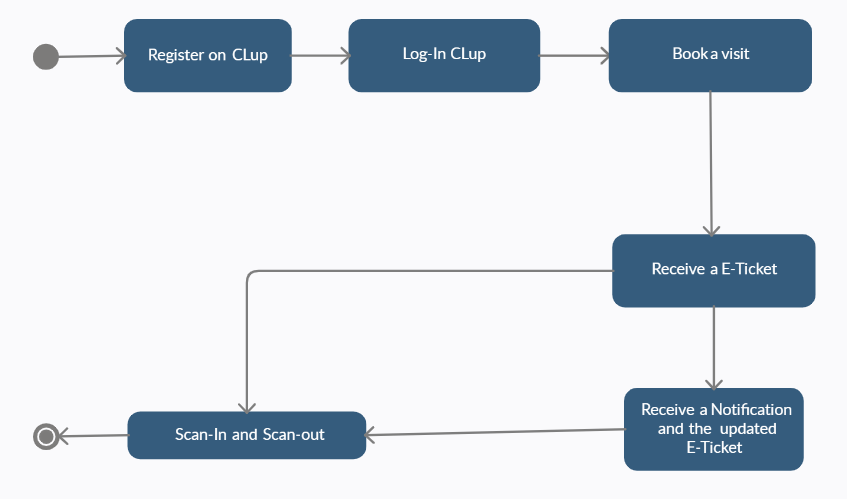
\includegraphics[scale=0.3]{State_diagram1.png}
	\caption{Customer State Diagram}
	\centering
\end{figure}

\begin{figure} \label{State Diagram}
	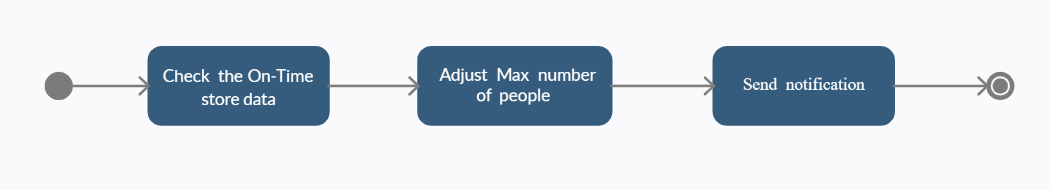
\includegraphics[scale=0.3]{State_diagram2.png}
	\caption{Store Manager State Diagram}
	\centering
\end{figure}

\begin{figure} \label{State Diagram}
	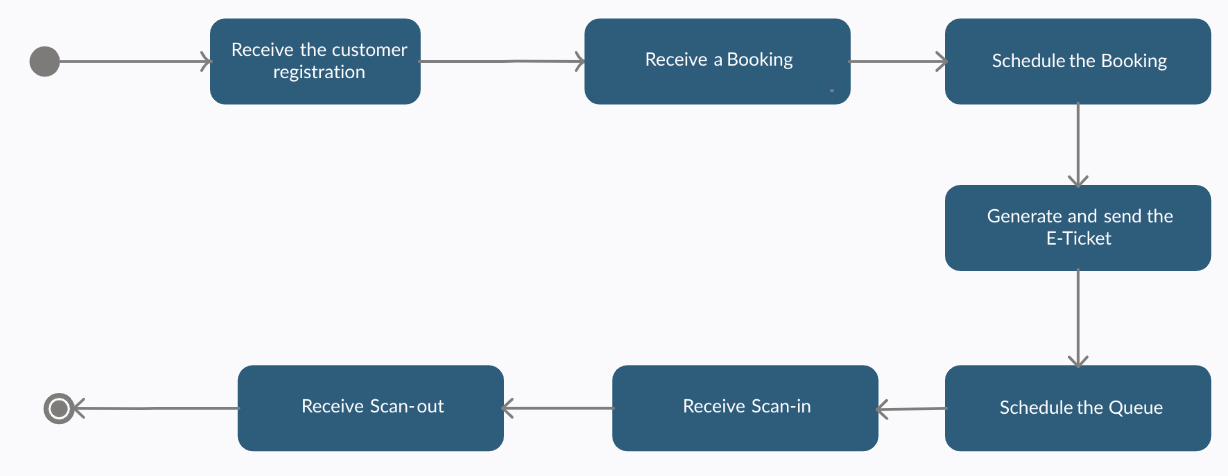
\includegraphics[scale=0.3]{State_diagram3.png}
	\caption{Server End State Diagram}
	\centering
\end{figure}


\begin{figure} \label{Class Diagram}
	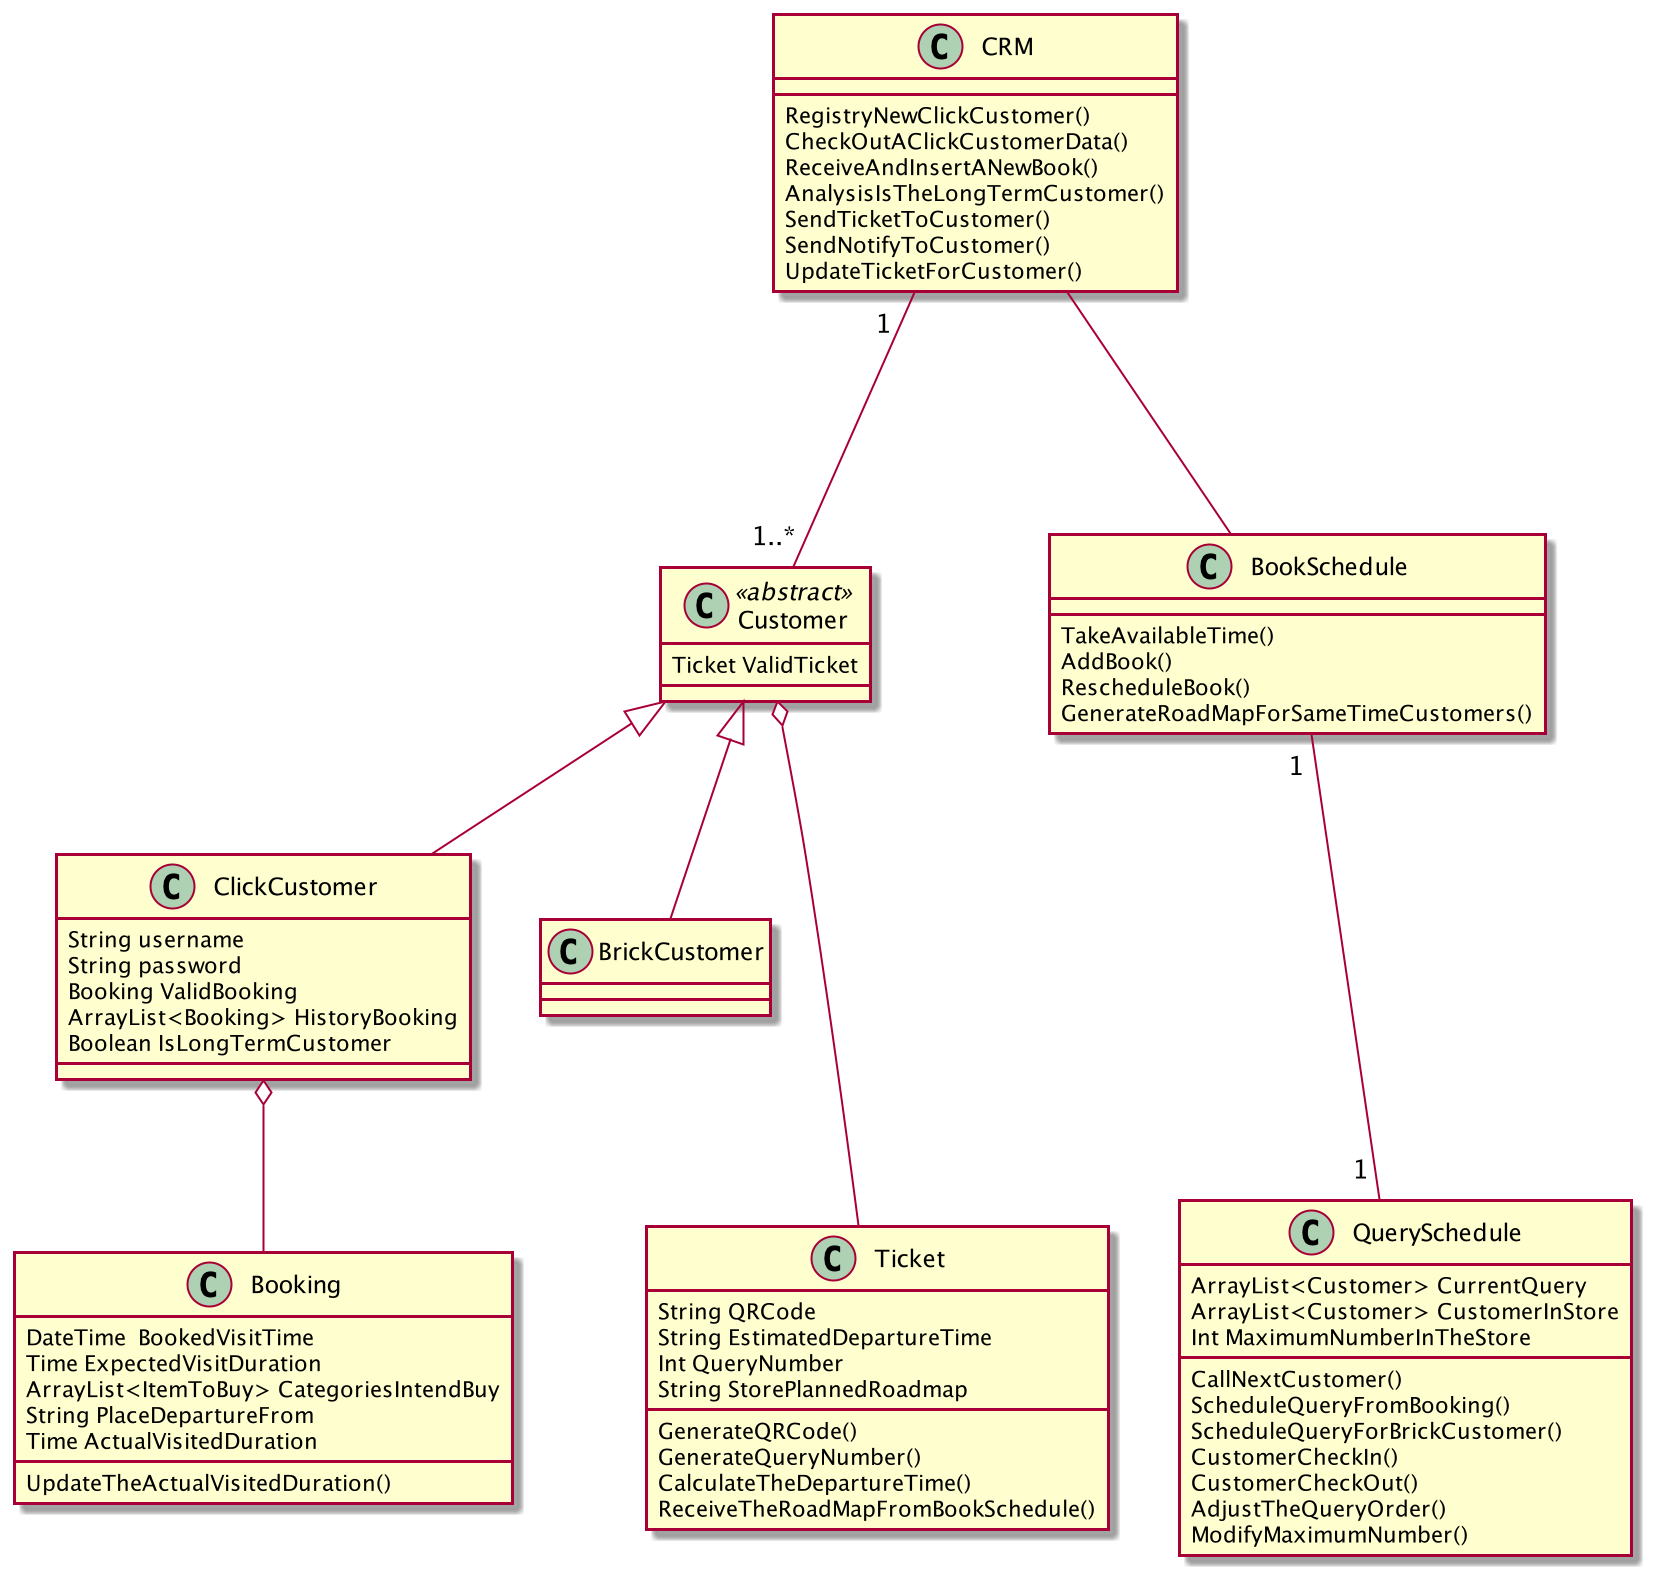
\includegraphics[scale=0.3]{class_diagram.png}
	\caption{CLup Class Diagram}
	\centering
\end{figure}



\section{Product functions}
\subsection{Functional Requirements}
\begin{itemize}
	\item Each \hyperref[Definitions]{Click Customer} shall be able to: 
	\begin{itemize}
		\item Sign-up 
		\item Login
		\item Book a visit,to complete it, they have to indicate the following data
		\begin{itemize}
			\item Indicate the desired date and time
			\item Indicate the approximate expected duration of the visit
			\item Indicate the categories of items that they intend to buy
			\item Indicate or given by GPS the current place they want to depart to the shop
		\end{itemize}
<<<<<<< HEAD
		\item Received the \hyperref[Definitions]{E-Ticket} with QR Code, the expected departure time and the queue number.
		\item Received a \hyperref[Definitions]{Store Path Map}.	
=======
		\item Received the \hyperref[Definitions]{E-Ticket} with QR Code, the estimated departure time and the queue number.
		\item Received a \hyperref[Definitions]{Store Planned Roadmap}.	
		\item Received the notification and the new E-ticket from store manager when their book is rescheduled.
>>>>>>> 811aecafafef745f71ead19af0ce42b7f2ab0f16
		\item The customer can scan the QR Code at \hyperref[Definitions]{QR Code scanned machine} when they enter \textbf{and} leave the store.
	\end{itemize}

	\item Each \hyperref[Definitions]{Brick Customer} shall be able to
	\begin{itemize}
		\item Retrieve the \hyperref[Definitions]{Ticket} from \hyperref[Definitions]{Tickets Hand-Out Machine} and wait the \hyperref[Definitions]{Digital Counterpart} call them.
		\item Scan the QR Code at QR Code Scanned Machine when they enter \textbf{and} leave the store.
	\end{itemize}

	\item \hyperref[Definitions]{Store Manager} shall be able to: 
	\begin{itemize}
		\item Check out the \hyperref[Definitions]{On-Time Store Data}
		\item Monitor the entrance QR code
		\item Hand out \hyperref[Definitions]{E-Ticket} for customer on the spot
	\end{itemize}

	\item The \hyperref[Definitions]{Store Back-End System} shall be able to:
	\begin{itemize}
		\item Send the available time/date to the the click customers.
		\item Received and schedule the click customers' book, the scheduling have to refer the duration time of each customer.
		\item Calculate the time from the click customer's departure place to the store,and put the estimated departure time on the E-Ticket.
		\item Plan and put the Store Planned Roadmap on the \hyperref[Definitions]{E-Ticket}
		\item Send the  E-Ticket to the click customers.
		\item Send a notification and new E-Ticket to the customer when their book is rescheduled.
		\item Store the customer's data,include:
		\begin{itemize}
			\item Username
			\item Password
			\item Valid Booking data
			\item History duration data
			\item Is long-term customers
		\end{itemize}
		\item Analysis the history duration data and sign the \hyperref[Definitions]{Long-Term Customers}.
		\item Calculate and store the \hyperref[Definitions]{On-Time Store Data}.
		\item Schedule the query from click customer's book and brick customer's retrieved ticket.
		\item Control the \hyperref[Definitions]{Digital Counterpart} and display the query number.
		\item Receive the information from the \hyperref[Definitions]{QR Code Scanned Machine}.
		\item Receive the information from the \hyperref[Definitions]{Tickets Hand-Out Machine}.
	\end{itemize}
\end{itemize}


\subsection{Non-Functional Requirements}
\begin{itemize}
	\item The time from the click customer's departure place to the store that calculate from the \hyperref[Definitions]{Store Back-End System} must enough precise to avoid the customer arriving at the the store too early/late.
	\item The Store Back-End System must schedule the query reasonably to minimize the wait time.
	\item The Store Back-End System must mix the book and brick customer's retrieved ticket reasonably to allow the click customers enter the store near the book time, by the way avoid making the brick customers wait too long.
	\item Cause of everyone needs to do grocery shopping, the software for the click customer should be enough simple to use,.
\end{itemize}

\section{User characteristics}

\section{Constraints}
There are not many constraints on customer's device, only need a smart phone with Android or IOS operation system, when they book a visit, the smartphone has to connect with internet, at other time, no need for a stable internet connection,only need to be able to connect to the Internet discontinuously to receive reminders that may appear.
The manager needs a PC with stable network connection.
For the \hyperref[Definitions]{Store Back-End System}, we buy a Amazon EC2 IaaS to implement this system.


\section{Assumptions, Dependencies}

\subsection{Domain Assumptions}
\begin{itemize}
	\item $D_1$ : Everyone will leave the departure place at the departure time indicated by the system.
	\item $D_2$ : Everyone who leaves on time can arrive at the store on time.
	\item $D_3$ : Everyone can leave the store in time according to their estimated time.
	\item $D_4$ : If something unexpected happens, the store manager can reschedule the customer's book reasonably.
	\item $D_5$ : If someone’s book is rescheduled, he can find the notification in time and set off according to the new ticket.
	\item $D_6$ : Everyone can consciously scan the QR code at the entrance and exit.
	\item $D_7$ : Everyone can follow the \hyperref[Definitions]{Planned Roadmap} in the store.
	\item $D_8$ : If is possible, everyone tries to best book the visit by the software(be a \hyperref[Definitions]{Click Customer}) instead of picking up tickets on the spot(not be a \hyperref[Definitions]{Brick Customer}).
\end{itemize}

\subsection{Goals}
There are only three main goals of this system.
\begin{itemize}
	\item $G_1$ : Allows store managers to regulate the influx of people in the building.
	\item $G_2$ : Saves people from having to line up and stand outside of stores for hours on end.
	\item $G_3$ : The application plan visits in a finer way to allow more people in the store, at the same time, let the customer occupy different spaces in the store to keep enough distance between them.
\end{itemize}

\chapter{Specific Requirements} \label{C3:SpecificRequirements}
\section{External Interface Requirements}
\subsection{User Interfaces}
\subsection{Hardware Interfaces}
\subsection{Software  Interfaces}
\subsection{Communication Interfaces}

\newpage
\section{Functional Requirements}
\subsection{User Class 1}
\subsubsection{Functional Requirement 1.1}
\subsection{User Class 2}
\subsubsection{Functional Requirement 2.1}

\newpage
\section{Performance Requirements}

\newpage
\section{Design Constraints}
\subsection{Standards compliance}
\subsection{Hardware limitations}

\newpage
\section{Software System Attributes}
\subsection{Reliability}
\subsection{Availability}
\subsection{Security}
\subsection{Maintainability}
\subsection{Portability}

\newpage
\section{Other Requirements}

\chapter{Formal Analysis Using Alloy}

\chapter{Effort Spent}

\begin{itemize}
	\item \textbf{Kong Xiangyi}
	\begin{center}
		\begin{tabular}{ |c|c|c| } 
			\hline
			Date & Task & Hours \\
			\hline
			\hline
			2020/10/10 & Group discussion project plan & 4h \\ 
			\hline
			2020/10/31 & Modified the purpose and scope of the RASD & 2h \\ 
			\hline
			2020/11/14 & Drawn the state diagram in the Section 2.1.1 & 2h \\ 
			\hline
		\end{tabular}
	\end{center}
	\item \textbf{Zhang Yuedong}
	\begin{center}
		\begin{tabular}{ |c|c|c| } 
			\hline
			Date & Task & Hours \\
			\hline
			\hline
			2020/10/10 & Group discussion project plan & 4h \\ 
			\hline
			2020/10/19 & Added the project's architecture & 1h \\ 
			\hline
			2020/10/30 & Added the purpose and scope of the RASD & 2h \\ 
			\hline
			2020/11/16 & Wrote the product functions part & 4h \\ 
			\hline
			2020/11/17 & Drawn the class diagram in the Section 2.1.1  & 2h \\ 
			\hline
		\end{tabular}
	\end{center}
\end{itemize}


\backmatter

\end{document}
